\chapter{Week 2: Higher-Order Functions, Scope, and State}
\label{ch:week2}

Lecture 2: September 15, 2026. Recitation 2: September 18, 2026.

Supplementary reading:
\begin{itemize}
  \item \cite{RacketGuide} Sections 4.4--4.6 (functions, local binding), 4.8 (sequencing), 5 (programmer-defined datatypes), and 12 (pattern matching).
  \item \cite{HtDP} Part II (self-referential data) and Part III (abstraction: \code{map}, \code{filter}, folds).
  \item \cite{SICP} Sections 1.3 (higher-order procedures) and 3.1 (assignment and local state).
\end{itemize}

Lecture~2 finishes the tour of Racket: more list recursion and accumulators, structs for tree-shaped data, functions as values, scope, and finally state. Recitation~2 then writes the first interpreter of the course, for Boolean expressions, together with an optimization pass. This chapter covers:
\begin{itemize}
  \item \Cref{sec:listsrec}: adding to the end of a list, a quadratic \code{reverse} and a broken one, and accumulators packaged as named \code{let};
  \item \Cref{sec:structs}: \code{struct}, binary trees, and \code{match};
  \item \Cref{sec:hof}: \code{lambda}, closures, \code{map}, \code{filter}, and the two folds;
  \item \Cref{sec:scopestate}: \code{let} and \code{let*}, lexical scope, pure code and side effects, and boxes;
  \item \Cref{sec:rec2}: Recitation~2, an interpreter and a De Morgan optimizer for Boolean expressions, and how to test an optimization.
\end{itemize}

\section{Lists and Accumulators}
\label{sec:listsrec}

Throughout this chapter we use the names \code{empty?}, \code{first}, and \code{rest} rather than \code{null?}, \code{car}, and \code{cdr}. They mean the same thing.

\subsection{\texttt{snoc}: Adding to the End}

\rkt|(cons x l)| makes one new pair whose head is \code{x} and whose tail is the old list \code{l}. Nothing is copied, so adding to the \emph{front} costs $O(1)$ however long the list is.

Adding to the \emph{back} is different. The old list ends in \code{'()}, and that \code{'()} cannot be replaced without rebuilding every pair on the way to it. So a back-insert walks the whole list, in $O(n)$. Racket does not provide one; we write it and call it \code{snoc}, ``cons'' backwards:

\begin{lstlisting}
(define (snoc l x)
  (cond
    [(empty? l) (list x)]
    [else (cons (first l) (snoc (rest l) x))]))
\end{lstlisting}

Two shapes of input, two branches: the skeleton of almost every list function in this course. The empty case answers ``the list containing just \code{x}''; the other keeps the first element in place and hands the rest of the problem to \code{snoc}. So \rkt|(snoc '() 'x)| is \code{'(x)} and \rkt|(snoc '(1 2) 'x)| is \code{'(1 2 x)}.

\subsection{Reversing, Correctly and Incorrectly}

To reverse a list, reverse everything after the first element, then put the first element at the very end, which is exactly \code{snoc}:
\begin{lstlisting}
(define (rev l)
  (cond
    [(empty? l) '()]
    [else (snoc (rev (rest l)) (first l))]))
\end{lstlisting}
\begin{lstlisting}[style=repl]
(rev '(1 2 3))
---> (snoc (rev '(2 3)) 1)
---> (snoc (snoc (rev '(3)) 2) 1)
---> (snoc (snoc '(3) 2) 1)
---> (snoc '(3 2) 1)
---> '(3 2 1)
\end{lstlisting}
This is correct but slow: one \code{snoc} per element, each $O(n)$, so $O(n^2)$ in total. It also needs $O(n)$ stack, because the \code{snoc} is wrapped \emph{around} the recursive call, which therefore is not a tail call.

Here is a tempting rewrite with \code{cons} instead of \code{snoc}:
\begin{lstlisting}
(define (rev-alt l)
  (cond
    [(empty? l) '()]
    [else (cons (rev-alt (rest l)) (first l))]))
\end{lstlisting}
\begin{lstlisting}[style=repl]
> (rev-alt '(1 2 3))
'(((() . 3) . 2) . 1)
\end{lstlisting}

\begin{pitfall}[\code{cons} is not symmetric]
\code{cons} expects an element on the left and a list on the right. \code{rev-alt} passes them the other way round, so it builds a nest of pairs, not a list (\Cref{fig:revalt}). There is no error, because a pair may hold any two values: the wrong argument order is a \emph{silent} bug, and the dots in the output are the only sign. Swapping the arguments does not rescue this approach: \code{cons} can only ever add to the front, and reversing needs to add to the back.
\end{pitfall}

\begin{figure}[htbp]
\centering
\begin{tikzpicture}[x=1cm, y=1cm]
  \node[cell] (a1) at (0,0) {}; \node[cell, right=0pt of a1] (d1) {};
  \node[cell] (a2) at (-1.6,-1.3) {}; \node[cell, right=0pt of a2] (d2) {};
  \node[cell] (a3) at (-3.2,-2.6) {}; \node[cell, right=0pt of a3] (d3) {};
  \node (one) at (1.0,-1.1) {\code{1}};
  \node (two) at (-0.6,-2.4) {\code{2}};
  \node (three) at (-2.2,-3.7) {\code{3}};
  \draw[ptr] (a1.center) -- (d2.north);
  \draw[ptr] (a2.center) -- (d3.north);
  \draw[ptr] (d1.center) -- (one);
  \draw[ptr] (d2.center) -- (two);
  \draw[ptr] (d3.center) -- (three);
  \draw (a3.south west) -- (a3.north east);
  \node[right=10mm of d1, lbl, align=left] {\code{'(((() . 3) . 2) . 1)}:\\ the \emph{car}s chain, the \emph{cdr}s hold elements};
\end{tikzpicture}
\caption{What \code{rev-alt} builds: every pair has a non-list on its right, hence the dots.}
\label{fig:revalt}
\end{figure}

\subsection{Aggregating a List}

Summing a list follows the same skeleton:
\begin{lstlisting}
(define (sum-list l)
  (cond
    [(empty? l) 0]
    [else (+ (first l) (sum-list (rest l)))]))
\end{lstlisting}
The \code{+} sits \emph{outside} the recursive call. It cannot happen until the recursion returns, so every level must be remembered, and a long enough list runs out of stack.

As with \code{fact} in \Cref{sec:exprrec}, the fix is to carry the running total as an extra argument, making the recursive call a tail call:
\begin{lstlisting}
(define (sum-list-helper l acc)
  (cond
    [(empty? l) acc]
    [else (sum-list-helper (rest l) (+ (first l) acc))]))

(define (sum-list-acc l)
  (sum-list-helper l 0))
\end{lstlisting}
\begin{lstlisting}[style=repl]
(sum-list-helper '(1 2 3) 0)
---> (sum-list-helper '(2 3) 1)
---> (sum-list-helper '(3) 3)
---> (sum-list-helper '() 6)
---> 6
\end{lstlisting}

\subsection{Named \texttt{let}: Hiding the Helper}

A top-level helper with an extra argument is noise. A \emph{named \code{let}} packages the same thing as a loop: the name after \code{let} becomes a local function, and the bindings give its parameters and their starting values.
\begin{lstlisting}
(define (sum-list-loop l)
  (let loop ([l l]
             [acc 0])
    (cond
      [(empty? l) acc]
      [else (loop (rest l) (+ (first l) acc))])))
\end{lstlisting}
This is the idiomatic way to write a loop in Racket; it runs exactly like the helper version.

\section{Structs and Trees}
\label{sec:structs}

\subsection{\texttt{struct}}

\code{struct} defines a new kind of compound value. One line
\begin{lstlisting}
(struct bt (label left right) #:transparent)
\end{lstlisting}
generates five functions:
\begin{itemize}
  \item \code{bt}, the constructor: \rkt|(bt 1 empty empty)|;
  \item \code{bt?}, a predicate that answers \code{\#t} for these values;
  \item \code{bt-label}, \code{bt-left}, \code{bt-right}, the accessors for the three fields.
\end{itemize}

\begin{pitfall}[Forgetting \code{\#:transparent}]
Without \code{\#:transparent}, a struct value prints as \code{\#<bt>} with its contents hidden, and \code{equal?} is true only when the two values are the very same object. Two trees that look identical then compare as different, and every test that compares trees fails. With the flag, values print readably and \code{equal?} compares field by field.
\end{pitfall}

\code{struct} does \emph{not} check the types of its fields. \rkt|(bt 1 2 3)| is accepted, even though 2 and 3 are not trees. Nothing goes wrong until some traversal calls \code{bt-label} on the number 2, possibly far from the line that built the bad value. \Cref{sec:definetype} returns to this point: \code{define-type} in \code{plai-typed} rejects such a value where it is built.

\subsection{Binary Trees}

The empty tree is represented by \code{'()}, so a binary tree is either \code{empty} or a \code{bt} with a label and two subtrees.
\begin{lstlisting}
(define tree
  (bt 1
      (bt 2 empty empty)
      (bt 3 empty empty)))
\end{lstlisting}

The definition of a tree mentions trees in \emph{two} places, left and right, so a function over trees has two recursive calls. Lists mentioned themselves once, and list functions had one. The shape of the code follows the shape of the data (\Cref{fig:bt}).

\begin{lstlisting}
(define (sum-bt t)
  (cond
    [(empty? t) 0]
    [(bt? t) (+ (bt-label t)
                (sum-bt (bt-left t))
                (sum-bt (bt-right t)))]
    [else (error 'sum-bt "not a tree: ~a" t)]))
\end{lstlisting}

\begin{figure}[htbp]
\centering
\begin{tikzpicture}[level distance=11mm, sibling distance=24mm,
    every node/.style={ast}, level 2/.style={sibling distance=12mm}]
  \node {bt 1}
    child {node {bt 2} child {node[astl] {'()}} child {node[astl] {'()}}}
    child {node {bt 3} child {node[astl] {'()}} child {node[astl] {'()}}};
\end{tikzpicture}
\hspace{1.2cm}
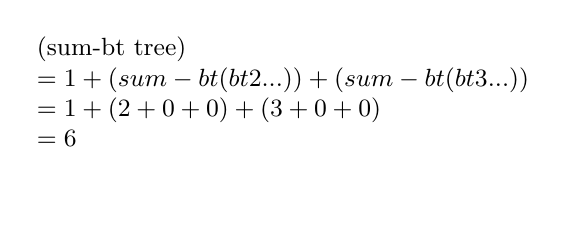
\begin{tikzpicture}[baseline=-14mm]
  \node[draw=none, fill=none, align=left, font=\small] {
    \code{(sum-bt tree)}\\
    $= 1 + \code{(sum-bt (bt 2 ...))} + \code{(sum-bt (bt 3 ...))}$\\
    $= 1 + (2 + 0 + 0) + (3 + 0 + 0)$\\
    $= 6$};
\end{tikzpicture}
\caption{The value \code{tree}. Each \code{bt} node causes two recursive calls, one per subtree.}
\label{fig:bt}
\end{figure}

Tree recursion is usually not made tail-recursive: with two recursive calls, at most one of them can be the last thing the function does, and the other has to be remembered.

\subsection{\texttt{match}}

\code{match} checks the shape and extracts the fields in one step, which reads better once all the fields are needed anyway:
\begin{lstlisting}
(define (sum-bt/match t)
  (match t
    ['() 0]
    [(bt label left right)
     (+ label (sum-bt/match left) (sum-bt/match right))]))
\end{lstlisting}
The pattern \rkt|(bt label left right)| matches only \code{bt} values and binds the three names to the fields in order.

\subsection{(SUPPLEMENT) Further Topics}

\subsubsection{Structural recursion} Functions like \code{sum-bt} are \emph{structurally recursive}: they recur only on immediate sub-parts of their input. Such functions always terminate on finite data, since each call is on a strictly smaller value, and their correctness can be proved by \emph{structural induction}, one case per variant. Every interpreter in this course is structurally recursive in its \code{eval} on the abstract syntax tree, except where substitution builds a new tree (\Cref{ch:week4}).

\subsubsection{Opaque structs and abstraction} Opacity is the default for a reason: an opaque struct hides its representation, so a module can export the struct without letting clients inspect or compare its insides. Transparent structs are the right choice for plain data such as trees and syntax, where structural equality is what you want. A middle ground is \code{\#:prefab}, which also makes structs readable and writable as literals.

\subsubsection{Contracts on fields} Plain Racket can check field types at run time with \code{struct/contract} or \code{contract-out}, e.g.\ requiring \code{left} to satisfy \code{(or/c empty? bt?)}. The error then points at the bad construction rather than the later traversal. \code{plai-typed} (\Cref{ch:week3}) instead checks before the program runs.

\section{Higher-Order Functions}
\label{sec:hof}

\subsection{Functions Are Values}

A function does not need a name. \code{lambda} builds one on the spot, and it can be called immediately: \rkt|((lambda (x) (* x x)) 4)| is \code{16}. So \code{define} for functions is shorthand, and these two definitions are the same:
\begin{lstlisting}
(define (square x)
  (* x x))

(define square-alt
  (lambda (x) (* x x)))
\end{lstlisting}
Use the short form. Do not nest one form inside the other: \rkt|(define (f x) (lambda ...))| defines a function that \emph{returns} a function, which is a different thing.

Since functions are values, a function can return one:
\begin{lstlisting}
(define (make-adder x)
  (lambda (y) (+ x y)))

(define add2 (make-adder 2))
\end{lstlisting}

\begin{definition}[Closure]
A \emph{closure} is a function value together with the bindings of the variables it refers to from the surrounding code.
\end{definition}

\rkt|(make-adder 2)| returns a function that has not been called yet but already remembers that \code{x} is 2. Then \rkt|(add2 5)| is 7, and \rkt|((make-adder 3) 4)| is 7 as well.

\subsection{\texttt{map} and \texttt{filter}}

Once functions can be arguments, the two most common list patterns become ordinary functions. \code{map} applies a function to every element; the result has the same length as the input.
\begin{lstlisting}
(define (my-map f l)
  (cond
    [(empty? l) '()]
    [else (cons (f (first l)) (my-map f (rest l)))]))
\end{lstlisting}
So
\begin{lstlisting}
(map f (list a b c))                       ; = (list (f a) (f b) (f c))
(map (lambda (x) (+ 1 x)) (list 1 2 3))    ; = '(2 3 4)
\end{lstlisting}

\code{filter} keeps the elements that pass a test; the contents are unchanged, only the length shrinks. To drop an element, return the filtered rest without \code{cons}ing it back on:
\begin{lstlisting}
(define (my-filter f l)
  (cond
    [(empty? l) '()]
    [else (if (f (first l))
              (cons (first l) (my-filter f (rest l)))
              (my-filter f (rest l)))]))
\end{lstlisting}
\rkt|(filter odd? (list 1 2 3 4 5))| is \code{'(1 3 5)}.

\begin{keypoint}[Three shapes of list code]
\code{map}: list to list, same length. \code{filter}: list to list, shorter. \code{fold}: list to a single value. Most list code is a combination of these three.
\end{keypoint}

\subsection{Folds}

\code{map} and \code{filter} each fix what happens at every step. A \emph{fold} takes the step as an argument: a two-argument \code{combine}, a \code{base} value for the empty list, and the list. It walks the list once and collapses it into one value. There are two folds, and they differ in which way the parentheses group (\Cref{fig:folds}):
\begin{align*}
\code{(my-foldl - 0 '(1 2 3))} &= ((0 - 1) - 2) - 3 = -6, \\
\code{(my-foldr - 0 '(1 2 3))} &= 1 - (2 - (3 - 0)) = 2.
\end{align*}
With an associative and commutative \code{combine} such as \code{+}, \code{*}, or \code{max}, the two agree, which is why the difference is easy to miss until it bites.

\begin{figure}[htbp]
\centering
\begin{tikzpicture}[level distance=9mm, sibling distance=9mm, every node/.style={ast}]
  \node[asth] {-}
    child {node[asth] {-}
      child {node[asth] {-} child {node[astl] {0}} child {node {1}}}
      child {node {2}}}
    child {node {3}};
  \node[draw=none, fill=none, font=\small] at (0,-4.0) {\code{foldl}: $((0-1)-2)-3$};
\end{tikzpicture}
\hspace{2cm}
\begin{tikzpicture}[level distance=9mm, sibling distance=9mm, every node/.style={ast}]
  \node[asth] {-}
    child {node {1}}
    child {node[asth] {-}
      child {node {2}}
      child {node[asth] {-} child {node {3}} child {node[astl] {0}}}};
  \node[draw=none, fill=none, font=\small] at (0,-4.0) {\code{foldr}: $1-(2-(3-0))$};
\end{tikzpicture}
\caption{The two folds of \code{-} over \code{'(1 2 3)} with base 0 (green). \code{foldl} leans left, starting from the base; \code{foldr} leans right, ending at the base.}
\label{fig:folds}
\end{figure}

\subsubsection{\code{foldl} combines on the way down} In \code{my-foldl}, \code{base} doubles as the running accumulator. Each step folds one more element into it and calls itself, and that call is a tail call, so this is a loop in constant stack space:
\begin{lstlisting}
(define (my-foldl combine base l)
  (cond
    [(empty? l) base]
    [else (my-foldl combine (combine base (first l)) (rest l))]))
\end{lstlisting}
\begin{lstlisting}[style=repl]
(my-foldl + 0 '(1 2 3 4 5))
---> (my-foldl + 1 '(2 3 4 5))
---> (my-foldl + (+ 1 2) '(3 4 5))
---> (my-foldl + (+ 3 3) '(4 5))
---> (my-foldl + (+ 6 4) '(5))
---> (my-foldl + 15 empty)
---> 15
\end{lstlisting}
Nothing is pending; at every step the accumulator is a value and the list is shorter.

\subsubsection{\code{foldr} combines on the way back up} In \code{my-foldr}, \code{combine} wraps the recursive call. No arithmetic can happen until the recursion reaches \code{'()} and the base value comes back:
\begin{lstlisting}
(define (my-foldr combine base l)
  (cond
    [(empty? l) base]
    [else (combine (first l) (my-foldr combine base (rest l)))]))
\end{lstlisting}
\begin{lstlisting}[style=repl]
(my-foldr + 0 '(1 2 3 4 5))
---> (+ 1 (my-foldr + 0 '(2 3 4 5)))
---> (+ 1 (+ 2 (my-foldr + 0 '(3 4 5))))
---> (+ 1 (+ 2 (+ 3 (+ 4 (+ 5 (my-foldr + 0 empty))))))
---> (+ 1 (+ 2 (+ 3 (+ 4 (+ 5 0)))))
---> 15
\end{lstlisting}
That growing pile of pending additions \emph{is} the stack: it is the concrete reason \code{foldr} uses $O(n)$ space and \code{foldl} $O(1)$.

\begin{keypoint}[\code{foldr} rebuilds structure]
\rkt|(my-foldr cons '() l)| copies \code{l}, because \code{foldr} replaces each \code{cons} of the list by \code{combine} and the final \code{'()} by \code{base}. Hence \code{map} and \code{filter} are both folds in disguise:
\begin{lstlisting}
(define (map-as-fold f l)
  (my-foldr (lambda (x acc) (cons (f x) acc)) '() l))

(define (filter-as-fold f l)
  (my-foldr (lambda (x acc) (if (f x) (cons x acc) acc)) '() l))
\end{lstlisting}
\end{keypoint}

\begin{pitfall}[Racket's \code{foldl} argument order]
The \code{combine} of \code{my-foldl} takes \code{(acc elem)}. Racket's built-in \code{foldl} calls \code{(combine elem acc)}, element first, the opposite order. So \rkt|(foldl - 0 '(1 2 3))| in Racket is $3-(2-(1-0)) = 2$, not $-6$. Check the order before reusing a \code{combine}.
\end{pitfall}

\section{Scope and State}
\label{sec:scopestate}

\subsection{\texttt{let} and \texttt{let*}}

\code{let} binds names to values for the extent of its body. The clauses go in one pair of brackets; square and round brackets are interchangeable in Racket, so both of these are the same form:
\begin{lstlisting}
(let ([x (+ 1 2)])
  (+ x x))            ; 6

(let [(x (+ 1 2))
      (y (+ 4 5))]
  (+ x y))            ; 12
\end{lstlisting}

The catch is \emph{when} each name starts to exist. \code{let} evaluates all of its right-hand sides first, in the scope \emph{outside} the \code{let}, and only then binds the names. So a later clause cannot use an earlier one:
\begin{lstlisting}
(let ([x (+ 1 2)]
      [y (+ 1 x)])     ; x is not bound here
  (+ x y))
;; x: undefined; cannot reference an identifier before its definition
\end{lstlisting}
Read the message as ``that name is not in scope here''.

\code{let*} binds the clauses one at a time, each in the scope of the previous ones, so this version works and gives 7:
\begin{lstlisting}
(define let-example
  (let* ([x (+ 1 2)]
         [y (+ 1 x)])
    (+ x y)))
\end{lstlisting}
There is no magic in \code{let*}; it is nested \code{let}s:
\[
\code{(let* ([x a] [y b]) body)} \quad\text{means}\quad \code{(let ([x a]) (let ([y b]) body))}.
\]
Use \code{let} by default, since it tells the reader the bindings are independent, and \code{let*} only when a clause really needs the one above it. Neither lets a clause refer to \emph{itself}: a local recursive function needs \code{letrec}, or the named \code{let} of \Cref{sec:listsrec}.

\subsection{Lexical Scope}

A \code{let} is an expression, so it can appear anywhere a value can, including in another \code{let}'s right-hand side:
\begin{lstlisting}
(define nested-let-example
  (let ([x (let ([y 3]) (+ y y))])
    (+ x x)))           ; x = 6, so 12
\end{lstlisting}
But \code{y} exists only inside the inner \code{let}. Writing \rkt|(+ x y)| in the outer body is the same undefined-identifier error, even though \code{y} was ``used'' a moment earlier (\Cref{fig:scope}).

\begin{figure}[htbp]
\centering
\begin{tikzpicture}[tok/.style={inner sep=1.5pt, font=\ttfamily\normalsize, anchor=base west}]
  \node[tok] (a1) at (0,0) {(let ([x};
  \node[tok, right=1mm of a1.base east, anchor=base west, draw, fill=uspace, rounded corners=2pt, inner sep=3pt] (inner) {(let ([y 3]) (+ y y))};
  \node[tok, right=0pt of inner.base east, anchor=base west] (a2) {])};
  \node[tok] (b1) at (0.6,-0.9) {(+ x};
  \node[tok, right=0pt of b1.base east, anchor=base west, text=sigc] (y) {\,y};
  \node[tok, right=0pt of y.base east, anchor=base west] (b2) {))};
  \begin{scope}[on background layer]
    \node[draw, fill=kspace!50, rounded corners=3pt, fit=(a1)(inner)(a2)(b2), inner sep=6pt] (outer) {};
  \end{scope}
  \node[lbl, right=3mm of a2] {scope of \code{y}: the green box};
  \node[lbl, right=3mm of b2, align=left] {scope of \code{x}: the body;\\ \code{y} is \emph{not} visible here};
\end{tikzpicture}
\caption{Scopes nest like the text. The body of the outer \code{let} is outside the inner \code{let}, so \code{y} is unbound there.}
\label{fig:scope}
\end{figure}

\begin{definition}[Lexical scope]
Under \emph{lexical} (static) scope, which binding a use of a name refers to is determined by where the binding is \emph{written} in the program text, not by what happened to run before.
\end{definition}

This is the same rule that makes the closure in \code{make-adder} work: the \code{x} in \code{(lambda (y) (+ x y))} refers to the \code{x} of the enclosing \code{define}, wherever the returned function is later called.

\subsection{Pure Code and Side Effects}

Everything so far is \emph{pure}: a call depends only on its arguments and does nothing but return a value. Run the same expression twice and you get the same answer, so an expression can always be replaced by its value without changing the program. That is what makes the step-by-step traces of \code{rev} and the folds valid reasoning, not just illustration.

A \emph{side effect} is anything else a call does: printing, mutating a variable, reading input, raising an error. In a language built on statements, \code{i++} is exactly this. Running it twice is not the same as running it once, so it cannot be replaced by its value.
\begin{itemize}
  \item \code{"Hello World"} is a value. Evaluating it does nothing else.
  \item \rkt|(print "Hello World")| writes to the console and returns \code{(void)}. The output is the point; the return value is not.
\end{itemize}
Racket does not forbid effects; it makes them ordinary expressions, so staying pure is a choice made function by function.

\subsubsection{Sequencing} A function body may hold several expressions. They run in order, the earlier ones only for their effects, and the value of the \emph{last} one is returned:
\begin{lstlisting}
(define (foo x)
  (print "Hello")
  (+ x 1))
\end{lstlisting}
\rkt|(foo 1)| returns 2 and prints along the way. The returned number is perfectly predictable; the printing is what makes \code{foo} impure. \code{begin} is the same sequencing as a single expression, for places where only one expression is allowed, such as a \code{cond} branch or an arm of \code{if}:
\begin{lstlisting}
(begin
  (print "Hello")
  (print "World")
  (+ 1 2))          ; returns 3, after printing
\end{lstlisting}

\subsubsection{Three ways to print} All return \code{(void)}; they differ only in what appears on the console. \rkt|(print "Hello")| shows \code{"Hello"}, the value as Racket would write it, quotes included. \rkt|(display "Hello")| shows \code{Hello}, the human-readable form. \rkt|(printf "The number foo is: ~a !" (* 3 3))| shows \code{The number foo is: 9 !}: \code{\textasciitilde a} splices in the display form of the next argument.

\subsection{Boxes: State You Can See}

A \emph{box} is a mutable container with exactly one slot, the smallest possible piece of state. It is a value like any other, so it can be passed to a function that changes it.
\begin{lstlisting}
(define bar (box 3))

(define (increment-box b)
  (set-box! b (+ 1 (unbox b))))
\end{lstlisting}
\rkt|(box 3)| makes a box, \rkt|(unbox bar)| reads it, and \rkt|(set-box! bar 10)| overwrites it and returns \code{(void)}. \code{increment-box} is called for its effect and returns nothing useful, so the caller has to \code{unbox} afterwards to see the new contents:
\begin{lstlisting}
(let ([b (box 3)])
  (increment-box b)
  (unbox b))          ; 4
\end{lstlisting}

The point of a box is that mutability is \emph{visible}. A plain 3 can never change; a box holding 3 announces that someone may change it, so a reader can tell where the state lives. By convention, a name ending in \code{!} mutates something: a warning that calling it twice is not the same as calling it once.

\section{Recitation 2: Boolean Expressions}
\label{sec:rec2}

This recitation builds the course's first interpreter and first program transformation, for a tiny language of Boolean expressions. Everything is in plain Racket, with structs and \code{match}.

\subsection{The Language and Its Representation}

The grammar of \emph{bexp}:
\[
\langle\textit{bexp}\rangle \;::=\; \langle\textit{boolean}\rangle \;\mid\; \langle\textit{bexp}\rangle \land \langle\textit{bexp}\rangle \;\mid\; \langle\textit{bexp}\rangle \lor \langle\textit{bexp}\rangle \;\mid\; \neg \langle\textit{bexp}\rangle
\]
One struct per alternative of the grammar represents it in Racket:
\begin{lstlisting}
(struct leaf-node (arg))
(struct or-node (left right))
(struct and-node (left right))
(struct not-node (arg))

(define bexp-bool-1 (and-node (leaf-node #t) (leaf-node #f)))
(define bexp-sym-1 (and-node (leaf-node 'x) (leaf-node 'y)))
\end{lstlisting}
A value built from these structs is an \emph{abstract syntax tree}: the tree structure replaces parentheses and precedence. Note that the structs are \emph{not} transparent and their fields are unchecked: \code{bexp-sym-1} has symbols, not booleans, at its leaves, and Racket accepts it.

\begin{exercise}[Syntactic equality]
Write \code{syn-equal?}, which checks whether two bexps are the same tree.
\end{exercise}
\begin{solution}
Because the structs are opaque, \code{equal?} would compare them by identity (\Cref{sec:structs}), so we write structural equality ourselves. \code{match*} matches several values at once, one pattern per value:
\begin{lstlisting}
(define (syn-equal? b1 b2)
  (match* (b1 b2)
    [((and-node l1 r1) (and-node l2 r2)) (and (syn-equal? l1 l2) (syn-equal? r1 r2))]
    [((or-node l1 r1) (or-node l2 r2))   (and (syn-equal? l1 l2) (syn-equal? r1 r2))]
    [((not-node a1) (not-node a2))       (syn-equal? a1 a2)]
    [((leaf-node v1) (leaf-node v2))     (equal? v1 v2)]
    [(_ _) #f]))
\end{lstlisting}
One clause per variant where both sides agree, and a final catch-all for mismatched shapes.
\end{solution}

\begin{pitfall}[A missing variant hides behind a catch-all]
If the \code{not-node} clause were left out, two \code{not-node}s would fall through to \rkt|[(_ _) #f]|, and \code{syn-equal?} would say a negation is not equal to itself. Nothing would complain, and every later test comparing expressions with a negation would fail even with a correct optimizer. With a catch-all clause present, check the list of variants, not just the clauses you were given.
\end{pitfall}

\subsection{An Interpreter for bexp}

\begin{exercise}[Interpreter]
Write \code{evaluate-bexp}, which computes the Boolean value an expression represents.
\end{exercise}
\begin{solution}
One clause per variant, and a recursive call wherever a variant contains a sub-expression:
\begin{lstlisting}
(define (evaluate-bexp b)
  (match b
    [(leaf-node v)    v]
    [(or-node b1 b2)  (or (evaluate-bexp b1) (evaluate-bexp b2))]
    [(and-node b1 b2) (and (evaluate-bexp b1) (evaluate-bexp b2))]
    [(not-node b1)    (not (evaluate-bexp b1))]))

(check-expect (evaluate-bexp (leaf-node #t)) #t)
(check-expect (evaluate-bexp (and-node (leaf-node #t) (leaf-node #f))) #f)
(check-expect (evaluate-bexp (and-node (leaf-node #f) (leaf-node #t))) #f)
\end{lstlisting}
The third test swaps the arguments of the second; testing both orders is cheap and catches an implementation that looks at only one side.
\end{solution}

This is the pattern of every interpreter in the course: our language's $\land$ is implemented by Racket's \code{and}, its $\lor$ by \code{or}, its $\neg$ by \code{not}. The \emph{meaning} of each construct is given by the clause that handles it.

\subsubsection{Missing cases} What happens with an incomplete \code{match}?
\begin{lstlisting}
(define (evaluate-bexp-m b)
  (match b
    [(leaf-node v) v]))
\end{lstlisting}
Nothing complains when it is defined. The error appears only when it is called on a value that no clause matches: \rkt|(evaluate-bexp-m bexp-bool-1)| raises \code{match: no matching clause}. Racket checks patterns at run time, so a missing case is found only if some test happens to reach it. \Cref{sec:rec3} redoes this in \code{plai-typed}, where the same mistake is rejected before the program runs.

\subsection{An Optimization Pass: De Morgan}

De Morgan's laws and double-negation elimination state the equivalences
\[
\neg(P \land Q) = \neg P \lor \neg Q, \qquad \neg(P \lor Q) = \neg P \land \neg Q, \qquad \neg\neg P = P.
\]
Using them left to right, an optimizer can eliminate redundant negations and push every remaining negation down to the leaves. The examples use symbolic leaves:
\begin{center}
\begin{tabular}{@{}lll@{}}
\toprule
name & before & after \\
\midrule
\code{bexp-1} & $\neg(\neg P \lor Q)$ & $P \land \neg Q$ \\
\code{bexp-2} & $\neg\neg P \lor \neg Q$ & $P \lor \neg Q$ \\
\code{bexp-3} & $P \lor \neg Q$ & $P \lor \neg Q$ (already optimal) \\
\bottomrule
\end{tabular}
\end{center}
\begin{lstlisting}
(define bexp-1 (not-node (or-node (not-node (leaf-node 'P)) (leaf-node 'Q))))
(define bexp-2 (or-node (not-node (not-node (leaf-node 'P))) (not-node (leaf-node 'Q))))
(define bexp-3 (or-node (leaf-node 'P) (not-node (leaf-node 'Q))))

(define bexp-1-opt (and-node (leaf-node 'P) (not-node (leaf-node 'Q))))
(define bexp-2-opt (or-node (leaf-node 'P) (not-node (leaf-node 'Q))))
(define bexp-3-opt (or-node (leaf-node 'P) (not-node (leaf-node 'Q))))
\end{lstlisting}

\subsubsection{What does it mean for an optimization to be correct?} Before writing the optimizer, decide how to check it. An optimization is correct when it does two things:
\begin{enumerate}
  \item it \emph{preserves semantics}: the output evaluates to the same value as the input;
  \item it actually \emph{optimizes}: the output has the promised shape, here every negation sitting directly on a leaf.
\end{enumerate}
Both become executable checks:
\begin{lstlisting}
(define (preserves-sem? unopt)
  (equal? (evaluate-bexp unopt) (evaluate-bexp (demorgan-opt unopt))))

(define (is-optimizing? opt)
  (define (only-not-at-leaves? bexp)
    (match bexp
      [(leaf-node v) #t]
      [(or-node b1 b2) (and (only-not-at-leaves? b1) (only-not-at-leaves? b2))]
      [(and-node b1 b2) (and (only-not-at-leaves? b1) (only-not-at-leaves? b2))]
      [(not-node (leaf-node v)) #t]
      [(not-node _) #f]))
  (only-not-at-leaves? opt))

(define (is-correct? unopt)
  (and (preserves-sem? unopt) (is-optimizing? (demorgan-opt unopt))))
\end{lstlisting}
\code{is-optimizing?} relies on \code{match} trying clauses in order: \rkt|(not-node (leaf-node v))| is tried first, so the catch-all \rkt|(not-node _)| sees only negations of compound expressions, which mean the pass left work undone. Note also that \code{preserves-sem?} takes only the input and calls \code{demorgan-opt} itself, so it tests the optimizer rather than a hand-written answer.

\subsubsection{The optimizer} What to do with a negation depends entirely on what is \emph{inside} it, so a single \rkt|(not-node b1)| clause cannot work. Nested patterns split it into the four shapes the argument can have, one per variant. This is what the handout means by ``you will need more cases than in \code{evaluate-bexp}'':
\begin{lstlisting}
(define (demorgan-opt b)
  (match b
    ; Standard Stuff
    [(leaf-node v)    (leaf-node v)]
    [(or-node b1 b2)  (or-node (demorgan-opt b1) (demorgan-opt b2))]
    [(and-node b1 b2) (and-node (demorgan-opt b1) (demorgan-opt b2))]
    [(not-node (leaf-node l)) (not-node (leaf-node l))]
    ; De-Morgan Stuff
    [(not-node (and-node b1 b2))
     (or-node (demorgan-opt (not-node b1)) (demorgan-opt (not-node b2)))]
    [(not-node (or-node b1 b2))
     (and-node (demorgan-opt (not-node b1)) (demorgan-opt (not-node b2)))]
    [(not-node (not-node b1)) (demorgan-opt b1)]))
\end{lstlisting}
\begin{itemize}
  \item \textbf{A negated leaf} is already as far down as a negation can go; keep it.
  \item \textbf{De Morgan.} After rewriting $\neg(b_1 \land b_2)$ to $\neg b_1 \lor \neg b_2$, the new negations may themselves sit on top of an \code{and}, an \code{or}, or a \code{not}, so they are optimized again: the recursive calls are on \rkt|(not-node b1)|, not on \code{b1}. Calling \rkt|(demorgan-opt b1)| would drop the negation and change the meaning.
  \item \textbf{Double negation.} The two negations cancel, and the result is \rkt|(demorgan-opt b1)|, not just \code{b1}, because \code{b1} may still contain negations to push down.
\end{itemize}

\begin{figure}[htbp]
\centering
\begin{tikzpicture}[level distance=9mm, sibling distance=14mm, every node/.style={ast}]
  \node[asth] {not}
    child {node {or}
      child {node[asth] {not} child {node[astl] {P}}}
      child {node[astl] {Q}}};
  \node[draw=none, fill=none, font=\small] at (0,-3.6) {$\neg(\neg P \lor Q)$};
\end{tikzpicture}
\hspace{0.8cm}
\begin{tikzpicture}
  \draw[arr] (0,0) -- (1.6,0) node[midway, above, lbl] {\code{demorgan-opt}};
  \node at (0,-1.6) {};
\end{tikzpicture}
\hspace{0.8cm}
\begin{tikzpicture}[level distance=9mm, sibling distance=14mm, every node/.style={ast}]
  \node {and}
    child {node[astl] {P}}
    child {node[asth] {not} child {node[astl] {Q}}};
  \node[draw=none, fill=none, font=\small] at (0,-3.6) {$P \land \neg Q$};
\end{tikzpicture}
\caption{\code{bexp-1} before and after the pass. Negations (yellow) end up only directly above leaves.}
\label{fig:demorgan}
\end{figure}

For \code{bexp-1} (\Cref{fig:demorgan}):
\begin{lstlisting}[style=repl]
(demorgan-opt (not (or (not P) Q)))
---> (and-node (demorgan-opt (not (not P))) (demorgan-opt (not Q)))   ; not over or
---> (and-node (demorgan-opt P) (not Q))                              ; not-not cancels
---> (and-node P (not Q))
\end{lstlisting}

\subsubsection{Why it terminates} Every recursive call is on a smaller tree. In the De Morgan cases the argument \rkt|(not-node b1)| is new, but it is smaller than the input \rkt|(not-node (and-node b1 b2))|, which has one more node and all of \code{b2} besides.

\subsection{Testing the Optimizer Two Ways}

The syntactic tests compare against the exact trees written by hand:
\begin{lstlisting}
(check-expect (syn-equal? (demorgan-opt bexp-1) bexp-1-opt) #t)
(check-expect (syn-equal? (demorgan-opt bexp-2) bexp-2-opt) #t)
(check-expect (syn-equal? (demorgan-opt bexp-3) bexp-3-opt) #t)
\end{lstlisting}
The semantic tests check the two correctness properties without writing the expected tree at all:
\begin{lstlisting}
(define bexp-4 (not-node (or-node (not-node (leaf-node #t)) (leaf-node #f))))
(define bexp-5 (or-node (not-node (not-node (leaf-node #t))) (not-node (leaf-node #f))))
(define bexp-6 (or-node (leaf-node #t) (not-node (leaf-node #t))))
(check-expect (is-correct? bexp-4) #t)
(check-expect (is-correct? bexp-5) #t)
(check-expect (is-correct? bexp-6) #t)
\end{lstlisting}

\begin{remark}[Why booleans at the leaves]
\code{bexp-4} to \code{bexp-6} are \code{bexp-1} to \code{bexp-3} with \code{\#t} and \code{\#f} in place of \code{'P} and \code{'Q}. With symbols at the leaves, \code{evaluate-bexp} is meaningless: \rkt|(not 'P)| is \code{\#f} and \rkt|(or 'P #f)| is \code{'P}, because Racket treats every value except \code{\#f} as true. So a semantic check only means something on Boolean leaves.
\end{remark}

\begin{remark}[The handout's table]
An earlier version of the handout listed $\neg(\neg P \land Q) \mapsto P \land Q$ as the first example. That contradicts both the code (\code{bexp-1} is built with \code{or-node}) and De Morgan's law; the posted solution corrects the row to $\neg(\neg P \lor Q) \mapsto P \land \neg Q$. Trust the definitions over the prose, and check the prose by working one example by hand.
\end{remark}

